\documentclass[14px]{article}
\usepackage{xeCJK}
\usepackage[frenchb]{babel}
\usepackage[T1]{fontenc}
\usepackage[utf8]{inputenc}
\usepackage{textcomp}
\usepackage{amssymb}
\usepackage[ruled,longend]{algorithm2e}
\usepackage{amsmath}
\usepackage{latexsym}
\usepackage{fancyhdr}
\usepackage{geometry}
\usepackage{setspace}
\renewcommand{\baselinestretch}{1.2}

\begin{document}
\setlength{\parindent}{0pt}
\begin{titlepage}

	\begin{center}
		% Upper part of the page
		
\includegraphics[width=0.35\textwidth]{logo.png}\\[1cm]

		\textsc{\Large Rapport de ALGAV}\\[0.5cm]

		% Title

		{ \huge \bfseries Caculer rectangle minimum convexe et cercle minimum convexe}\\[0.4cm]

		% Author and supervisor
		\begin{minipage}{0.4\textwidth}
			\begin{flushleft} \large
				\emph{Author:}\\
				Qiwei \textsc{XIAN}
			\end{flushleft}
		\end{minipage}
		\begin{minipage}{0.4\textwidth}
			\begin{flushright} \large
				\emph{Professeur:} \\
				Prof.\textsc{Bui-Xuan}
			\end{flushright}
		\end{minipage}

		\vfill
		% Bottom of the page
		{\large \today}
	\end{center}

\end{titlepage}
\clearpage

\tableofcontents
\thispagestyle{empty}
\clearpage

\pagestyle{fancy}
\lhead{Calculer le rectangle minimum convexe}
\rhead{\thepage}
\fancyfoot{}

\section{Préface}

\subsection{Objectif}
Dans ce projet, je vais présenter l'algorithme Toussaint et l'algorithme Ritter qui permet de calculer le rectangle minimum convexe et le cercle minimum convexe, en plus analyser leur performance ainsi que la qualité du rectangle minimum et le cercle minimum.

\subsection{Définition, notations, structures de données utilisées}
Calcule de vecteur
\begin{enumerate}
	\item $\overrightarrow{ab}$ est représenté le vecteur depuis $a$ vers $b$, $|\overrightarrow{ab}|$ est le scalaire de $\overrightarrow{ab}$.
	\item $\overrightarrow{ab}\cdot\overrightarrow{cd}$ dénote le produit scalaire entre $\vec{ab}$ et $\vec{cd}$.
	\item $\overrightarrow{ab}\times\overrightarrow{cd}$ dénote le produit vectoriel entre $\overrightarrow{ab}$ et $\overrightarrow{cd}$.
\end{enumerate}

On dénote l'ensembles de points par $\mathcal{P}$, le nombre de points de $\mathcal{P}$ par $n$.\\
Une enveloppe convexe $\mathrm{E}$ de $\mathcal{P}$ est un sous-ensemble $\mathrm{E}$ de $\mathcal{P}$ en ordre du sens horaire tel que le polygone composé par tous les points de $\mathrm{E}$ peut entourner tous les points de $\mathcal{P}$.\\
Un rectangle $Rec$ est représenté par une liste de quatre points. $RecMin$ est le rectangle minimum convexe. $AR$ est un ensemble de quatre arêtes de $Rec$.\\
Un cercle $Cer$ est représenté par un point du centre de cercle $O$ et le rayon $r$. $CerMin$ est le cercle minimum convexe.
\clearpage

\section{Algorithme Toussaint}
\subsection{Introduction}
Donner un ensemble $\mathcal{P}$ de n points dans $\mathbb{R}$, le rectangle minimum convexe est le rectangle qui entourne tous les points de $\mathcal{P}$ dont l'aire est la plus petite.\\\\
Calculer le rectangle minimum convexe est un des problèmes classiques de la géométrie algorithmique. Pour résoudre ce problème, un majorant de $\mathcal{O}(n^2)$ est donné par l'algorithm recherche exhaustive. Il existe aussi les autres meilleurs algorithmes comme \textbf{l'algorithme Shamos}, la première fois que Michael Shamos l'a utilisé afin de calculer la diamètre d’un polygone convexe en temps $\mathcal{O}(n)$ en 1978. En plus \textbf{l'algorithme Toussaint}, Godfried Toussaint a résolu beaucoup de problèmes de la géométrie algorithmique en utilisant la phase "\textbf{rotating caliper}". Dans mon projet, je cherche à calculer le rectangle minimum convexe en utilisant l'algorithme Toussaint.\\\\
Néanmoins il faut trouver l'enveloppe convexe de $\mathcal{P}$ avant d'utiliser ces algorithmes. Pour faire ce précalcule, il y a plusieurs choix possibles. Par exemple le \textbf{parcours de Graham}, il nous permet de calculer une enveloppe convexe en temps $\mathcal{O}(n\log n)$. Un autre algorithme la \textbf{marche de Jarvis}, il a aussi une excellente complexité en $\mathcal{O}(nh)$ où h représente le nombre de sommets de l'enveloppe convexe. \\\\
Dans ce projet, je choisis la marche de Jarvis afin de précalculer l'enveloppe convexe de $\mathcal{P}$. Dès qu’obtenir l'enveloppe, je vais utiliser rotating caliper pour chercher les autres points de l'enveloppe qui se trouve aussi dans le rectangle. Après je peux calculer les sommets de rectangle en utilisant ces quatre points. La complexité théorique est $\mathcal{O}(n + r)$ où r est la complexité de la marche de Jarvis.


\subsection{Présentation de l'algorithme Toussaint}
Afin de calculer les sommets A, B, C, D de rectangle, on a besoin d'abord de trouver $\alpha$ qui est colinéaire avec une arête de rectangle et les points $A^{\prime}$,  $B^{\prime}$, $C^{\prime}$, $D^{\prime}$ de $\mathcal{B}$ qui est sur les arêtes de $RecMin$.

\textbf{Lemma 1} if $Rec$ est $RecMin$, alors $\exists \mathcal{B}$, $\mathcal{B} \in \mathrm{E}$ tel que $\forall b, b \in \mathcal{B},\exists c, ar, c \in Rec, ar\in AR$, $\overrightarrow{bc}$ sont colinéaire avec $ar$.

\textbf{Lemma 2} il existe une arête $\alpha$ de $RecMin$, $\alpha$ passe une arête du polygone minimum convexe.


\subsubsection{Etape 1 calculer $A^{\prime}$,  $B^{\prime}$, $C^{\prime}$, $D^{\prime}$}
Pour $A^{\prime}$, on peut énumérer chaque point $i$ de $\mathrm{E}$, $A^{\prime} = E_{i}$,
et $\alpha = \overrightarrow{E_{i+1}E_{i}}$ \\

Pour $B^{\prime}$, il est le plus ouest point tel que $|\alpha \cdot \overrightarrow{B^{\prime}A^{\prime}}|$ est maximum, il exprime $\angle \alpha\overrightarrow{B^{\prime}A^{\prime}}$ est le plus grand. Comme $\mathrm{E}$ est en ordre du sens horaire, on énumère chaque point $E_{r}$ de $\mathrm{E}$, $|\alpha\cdot\overrightarrow{E_{r}A^{\prime}}| \leqslant |\alpha\cdot\overrightarrow{E_{r+1}A^{\prime}}|$, si une fois $|\alpha\cdot\overrightarrow{E_{r}A^{\prime}}| > |\alpha\cdot\overrightarrow{E_{r+1}A^{\prime}}|$, alors $B^{\prime} = E_{r}$\\

Pour $C^{\prime}$, il est le point antipodal de $A^{\prime}$, la distance entre $A^{\prime}$ et $C^{\prime}$ est plus grande que $A^{\prime}$ et les autres points, donc $|\alpha\times\overrightarrow{E_{u}A^{\prime}}|$ est maximum. Comme $\mathrm{E}$ est en ordre du sens horaire, si on énumère chaque point $E_{u}$ de $\mathrm{E}$, au début $|\alpha\times\overrightarrow{E_{u}A^{\prime}}| \leqslant |\alpha\times\overrightarrow{E_{u+1}A^{\prime}}|$, si une fois $|\alpha\times\overrightarrow{E_{u}A^{\prime}}| > |\alpha\times\overrightarrow{E_{u+1}A^{\prime}}|$, alors $C^{\prime}$ = $E_{u}$\\

Le dernier point $D^{\prime}$ est le plus est point, $\angle \alpha D^{\prime}$ est le plus petit. On énumère chaque point $E_{l}$ de $\mathrm{E}$, comme $\mathrm{E}$ est en ordre du sens horaire, au début $|\alpha\cdot\overrightarrow{E_{l}A^{\prime}}| \geq|\alpha\cdot\overrightarrow{E_{l+1}A^{\prime}}|$, si une fois $|\alpha\cdot\overrightarrow{E_{l}A^{\prime}}| < |\alpha\cdot\overrightarrow{E_{l+1}A^{\prime}}|$, alors $D^{\prime}$ = $E_{l}$\\

\subsubsection{Etape 2 calculer l'aire $\mathcal{S}$ de rectangle}
Pour la hauteur de rectangle $\mathrm{h}$, on suppose que le point $C^{\prime}_{\alpha}$ est le projecteur de $C^{\prime}$ sur $\alpha$, $\mathrm{h}= |\overrightarrow{C^{\prime}_{\alpha}C^{\prime}}|$
$\mathcal{S}_{\text{parallélogramme}}$ = $|\vec{\alpha}\times\overrightarrow{C^{\prime}A^{\prime}}|$. \\
$\mathrm{h} =  \frac{\mathcal{S}_{\text{parallélogramme}}}{|\vec{\alpha}|}$\\

Pour la largeur de rectangle $\mathrm{w}$, on suppose que $B^{\prime}_{\alpha}$ est le projecteur de $B^{\prime}$ sur $\alpha$ et $D^{\prime}_{\alpha}$ est le projecteur de $D^{\prime}$ sur $\alpha$, $\mathrm{w} = |\overrightarrow{B^{\prime}_{\alpha}D^{\prime}_{\alpha}}|$\\
$\overrightarrow{B^{\prime}_{\alpha}A^{\prime}}$ = $\frac{\alpha\cdot\overrightarrow{B^{\prime}A^{\prime}}}{|\alpha|}$\\
$\overrightarrow{D^{\prime}_{\alpha}A^{\prime}}$ = $\frac{\alpha\cdot\overrightarrow{D^{\prime}A^{\prime}}}{|\alpha|}$\\
$|\overrightarrow{B^{\prime}_{\alpha}D^{\prime}_{\alpha}}| = |\overrightarrow{D^{\prime}_{\alpha}A^{\prime}} - \overrightarrow{B^{\prime}_{\alpha}A^{\prime}}|$\\
Donc, $\mathcal{S} = h \times w$. Si $\mathcal{S} < \mathcal{S}_{RecMin}$, on va continuer à l'étape 3 afin de construire le nouveau $RecMin$ sinon on essaie le $A^{\prime}$ suivant.\\


\subsubsection{Etape 3 calculer $A$, $B$, $C$, $D$}
Dès qu’on obtient $A^{\prime}$,  $B^{\prime}$, $C^{\prime}$, $D^{\prime}$, $\alpha$, $\overrightarrow{B^{\prime}_{\alpha}A^{\prime}}$, $\overrightarrow{B^{\prime}_{\alpha}D^{\prime}_{\alpha}}$,
$\overrightarrow{C^{\prime}_{\alpha}C^{\prime}}$, on peut facilement calculer $A$, $B$, $C$, $D$.\\
$A$ est le point $B^{\prime}_{\alpha}$, $B^{\prime}_{\alpha} = A^{\prime} - \alpha\cdot\frac{\overrightarrow{B^{\prime}_{\alpha}A^{\prime}}}{|\alpha|}$\\
$B$ est le point suivant de $A$ au sens de horaire, $B =  B^{\prime}_{\alpha} +  \overrightarrow{B^{\prime}_{\alpha}B^{\prime}}\cdot\frac {\overrightarrow{C^{\prime}_{\alpha}C^{\prime}}}{|\overrightarrow{B^{\prime}_{\alpha}B^{\prime}}|}$\\
$C$ est le point suivant de $B$ au sens de horaire, $C = B + \overrightarrow{B^{\prime}_{\alpha}A^{\prime}}\cdot\frac{\overrightarrow{B^{\prime}_{\alpha}D^{\prime}_{\alpha}}}{|B^{\prime}_{\alpha}A{\prime}|}$\\
Le dernier point $D$ = $A - B$ = $C + \overrightarrow{BB^{\prime}_{\alpha}}$

\begin{algorithm}
	$\mathcal{P} \gets \text{Ensemble de points}$\;
	$\mathrm{E} \gets \text{Jarvis}(\mathcal{P})$\;
	$u \gets 1$\; $l \gets 1$\; $r \gets 1$\; $minAire \gets \infty$\;
	\For{$\textbf{each}\thinspace \text{arête} \thinspace \overrightarrow{E_{i+1}E_{i}},\thinspace 0\leqslant i < |E|$}{
		$A^{\prime} \gets E_{i}$\;
		$\alpha \gets \overrightarrow{E_{i+1}E_{i}}$\;
		\While{$|\alpha\times\overrightarrow{E_{u}E_{i}}| \leqslant |\alpha\times\overrightarrow{E_{u+1}E_{i}}|$}{
			$u \gets (u + 1)$ mod $|E|$\;
		}
		$C^{\prime} \gets E_{u}$\;
		\While{$|\alpha\cdot\overrightarrow{E_{r}E_{i}}| \leqslant |\alpha\cdot\overrightarrow{E_{r+1}E_{i}}|$}{
			$r \gets (r + 1)$ mod $|E|$\;
		}
		$B^{\prime} \gets E_{r}$\;
		\If{$i == 0$}{$l = r$\;}

		\While{$|\alpha\cdot\overrightarrow{E_{l}E_{i}}| \leqslant |\alpha\cdot\overrightarrow{E_{l+1}E_{i}}|$}{
			$l \gets (l + 1)$ mod $|E|$\;
		}
		$D^{\prime} \gets E_{l}$\;
		$\overrightarrow{B^{\prime}_{\alpha}A^{\prime}} \gets \thinspace$ $\frac{\alpha\cdot\overrightarrow{B^{\prime}A^{\prime}}}{|\alpha|}$\;

		$\overrightarrow{D^{\prime}_{\alpha}} \gets \thinspace$ $\frac{\alpha\cdot\overrightarrow{D^{\prime}A^{\prime}}}{|\alpha|}$\;

		$height \gets |C^{\prime}_{\alpha}C^{\prime}| \gets \thinspace$ $\frac{\alpha\times\overrightarrow{C^{\prime}A^{\prime}}}{|\alpha|}$\;

		$width \gets \overrightarrow{B^{\prime}_{\alpha}A^{\prime}} - \overrightarrow{D^{\prime}_{\alpha}A^{\prime}}$\;

		$aire \gets width\times height$\;
		\If{$aire < minAire$}{
			$minAire \gets aire$\;
			$A \gets A^{\prime} - \alpha\cdot \frac{\overrightarrow{B^{\prime}_{\alpha}A^{\prime}}}{|\alpha|}$\;
			$B \gets B^{\prime}_{\alpha} +  \overrightarrow{B^{\prime}_{\alpha}B^{\prime}}\cdot\frac {\overrightarrow{C^{\prime}_{\alpha}C^{\prime}}}{|\overrightarrow{B^{\prime}_{\alpha}B^{\prime}}|}$\;
			$C \gets B + \overrightarrow{B^{\prime}_{\alpha}A^{\prime}}\cdot\frac{\overrightarrow{B^{\prime}_{\alpha}D^{\prime}_{\alpha}}}{|B^{\prime}_{\alpha}A{\prime}|}$\;
			$D \gets C + (A - B)$\;
		}
	}
	\KwRet{$A, B, C, D$}\;
	\caption{Pseudocode de l'algorithme Toussaint}
\end{algorithm}

\subsection{Performance de l'algorithme}
Le graphe dessous est le temps d'exécution pour chaque teste de VAROUMAS.\\
{
	\centering
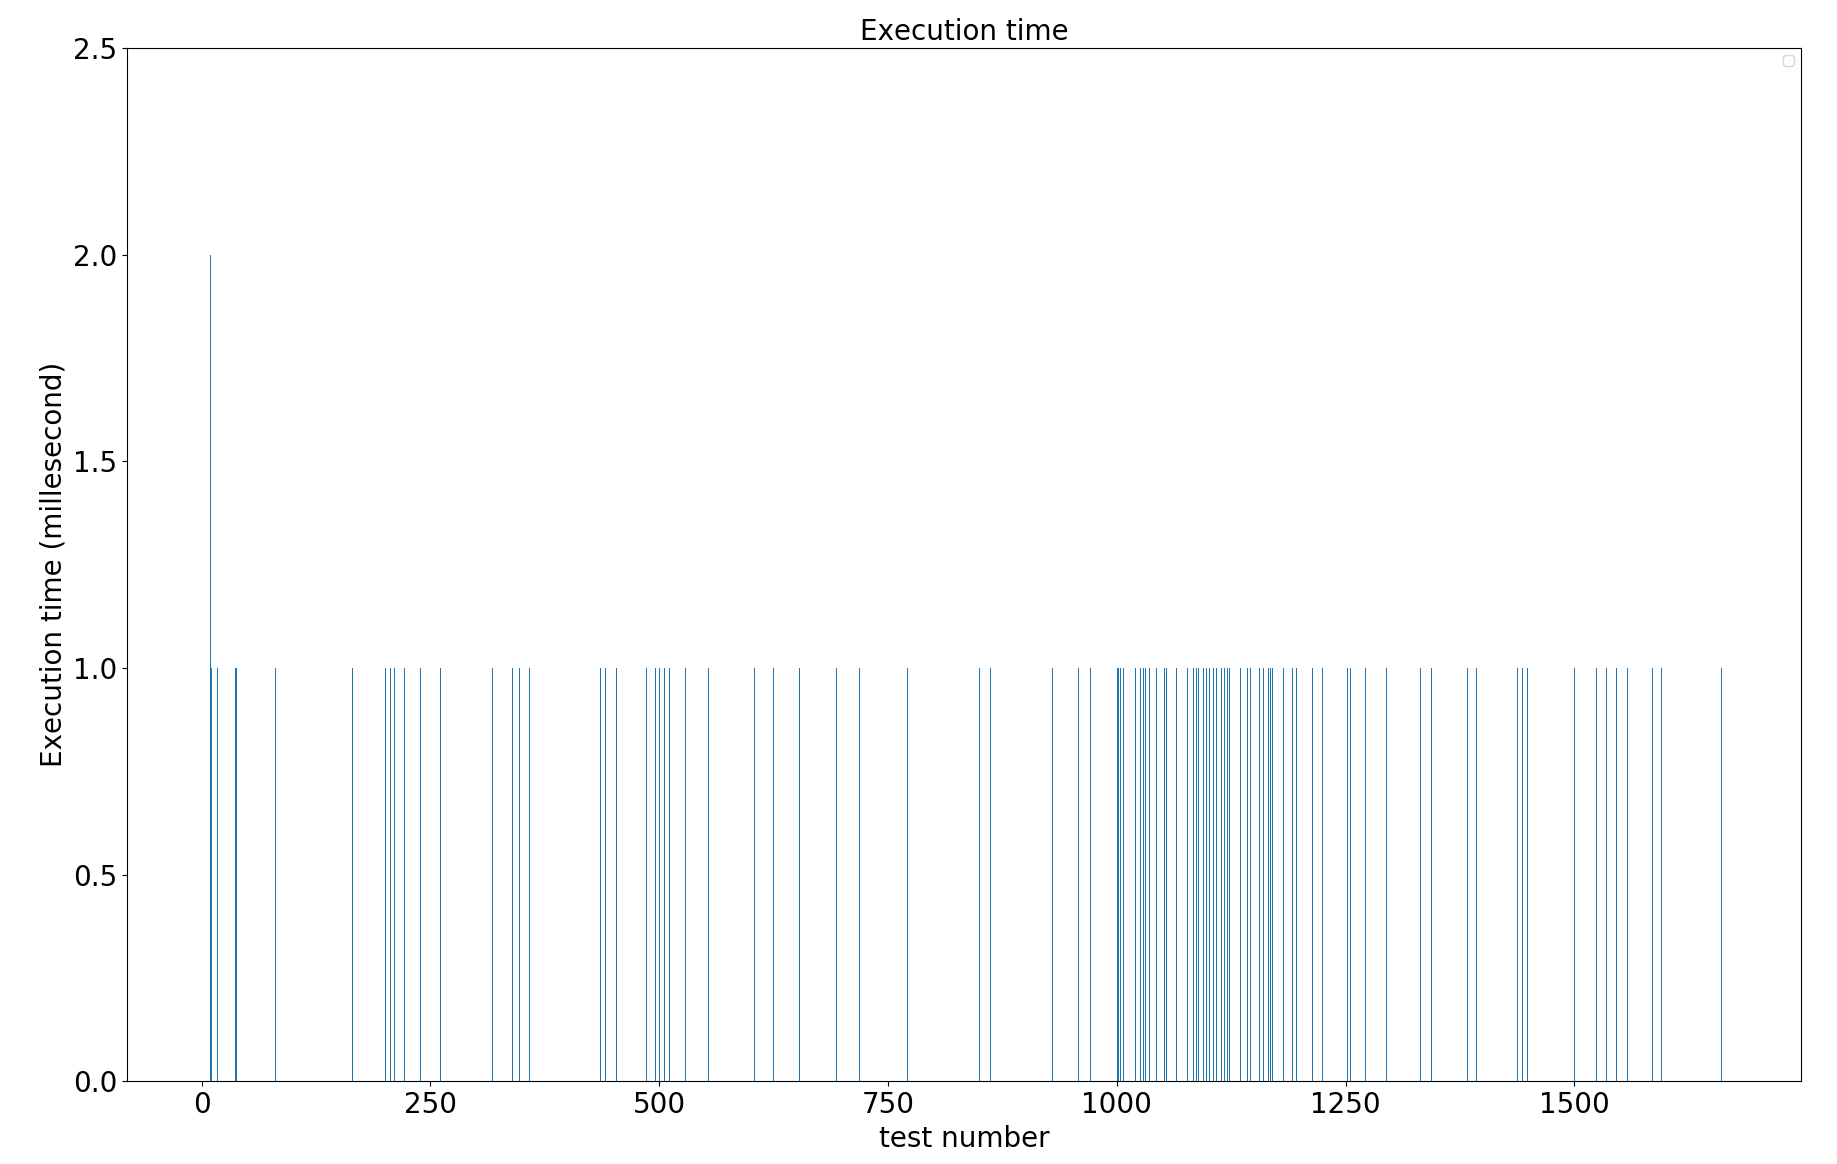
\includegraphics[height=0.5\textwidth]{testTime_Rectangle.png}\\
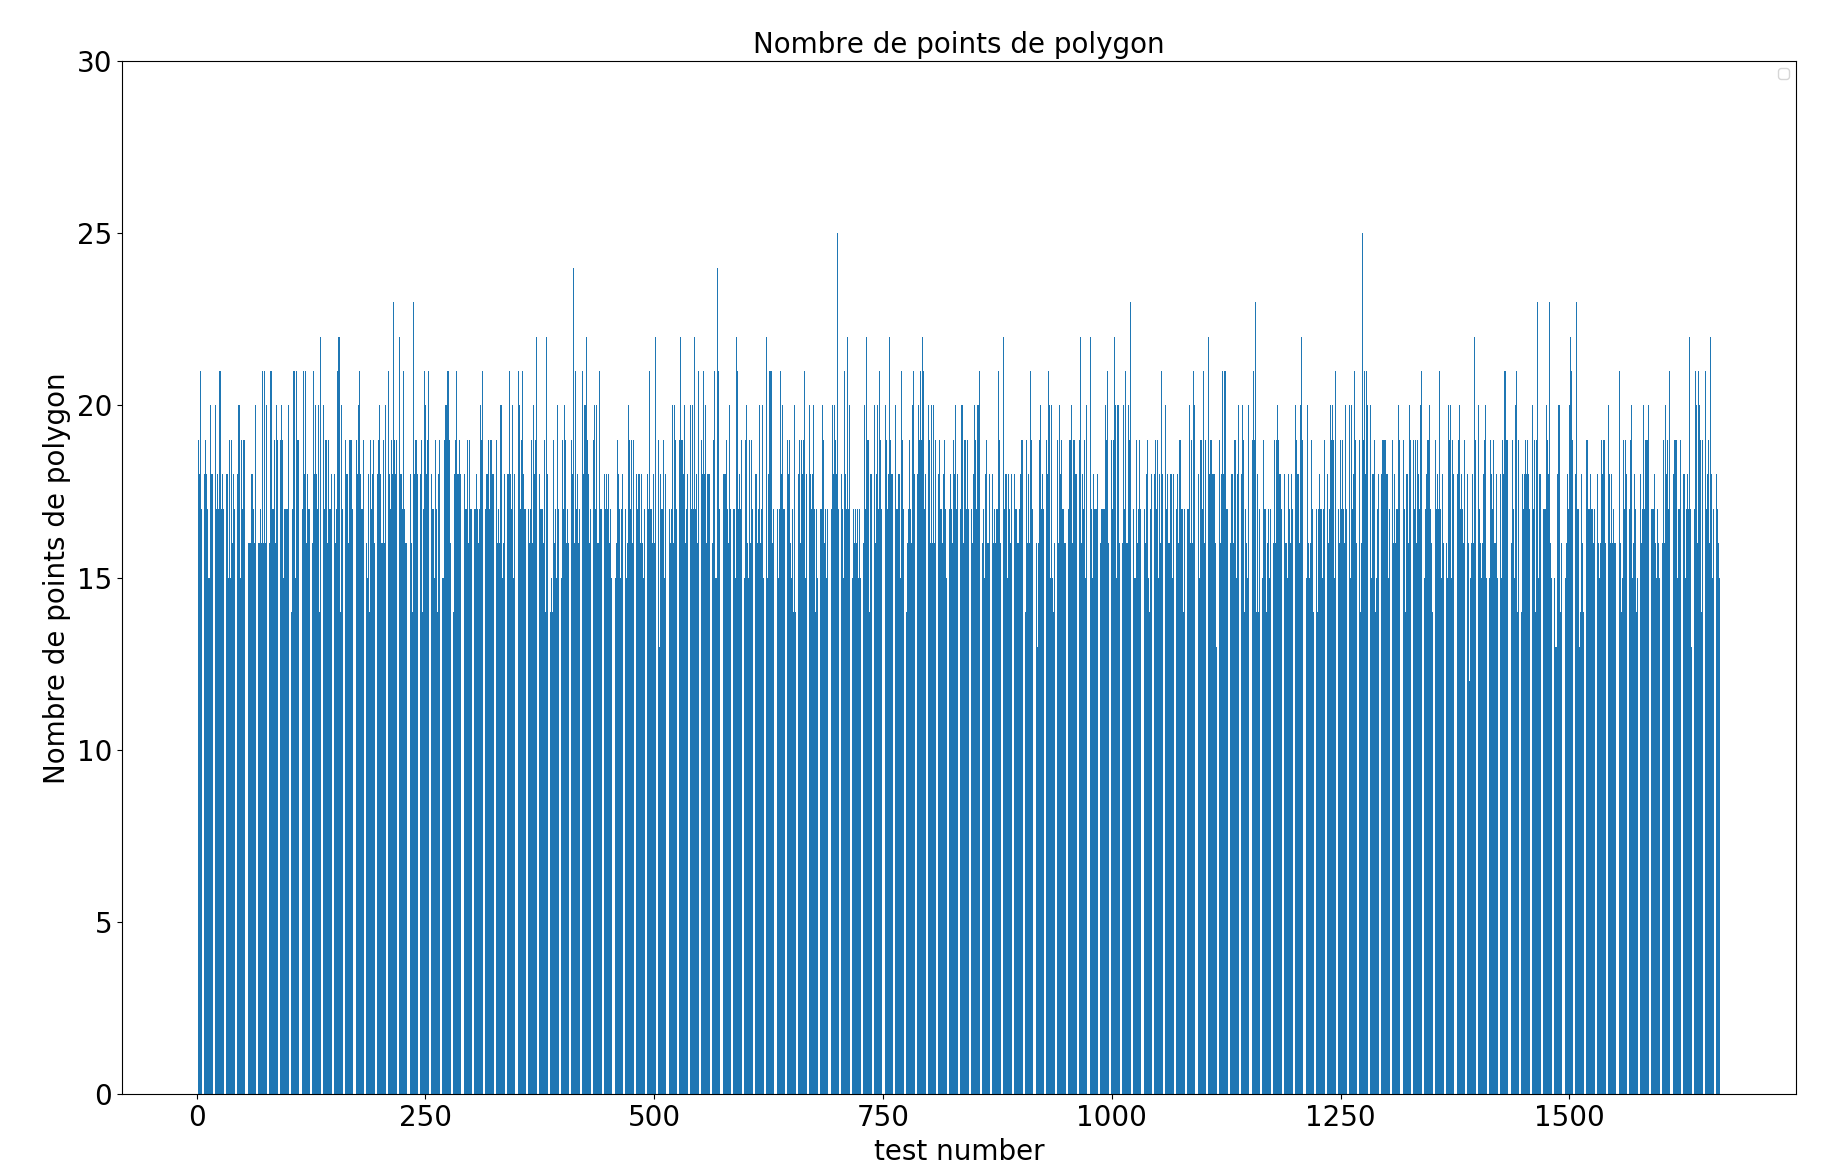
\includegraphics[height=0.5\textwidth]{testNombre.png}\\
}
Pour chaque cas de test, il y a 255 points aléatoire, après calculer l'enveloppe convexe en utilisant Jarvis, il reste seulement $\mathit{h}$ points de l'enveloppe convexe $ 12 \leqslant h \leqslant 25 $ dans tous les tests. En fonction de la complexité théorique de l'algorithme  $\mathcal{C} = \mathcal{O}(nh) + \mathcal{O}(h)$.
Donc le temps d'exécution n'est pas très évident. Pour la plupart de tests, le temps d'exécution $\mathit{t}$, $ 0 < \mathit{t} <= 1 ms$. Le test-10 prend le plus temps 2 ms.

\subsection{Résultat du test}
Le graphe dessous est le résultat de qualité associé à chaque teste de VAROUMAS.\\
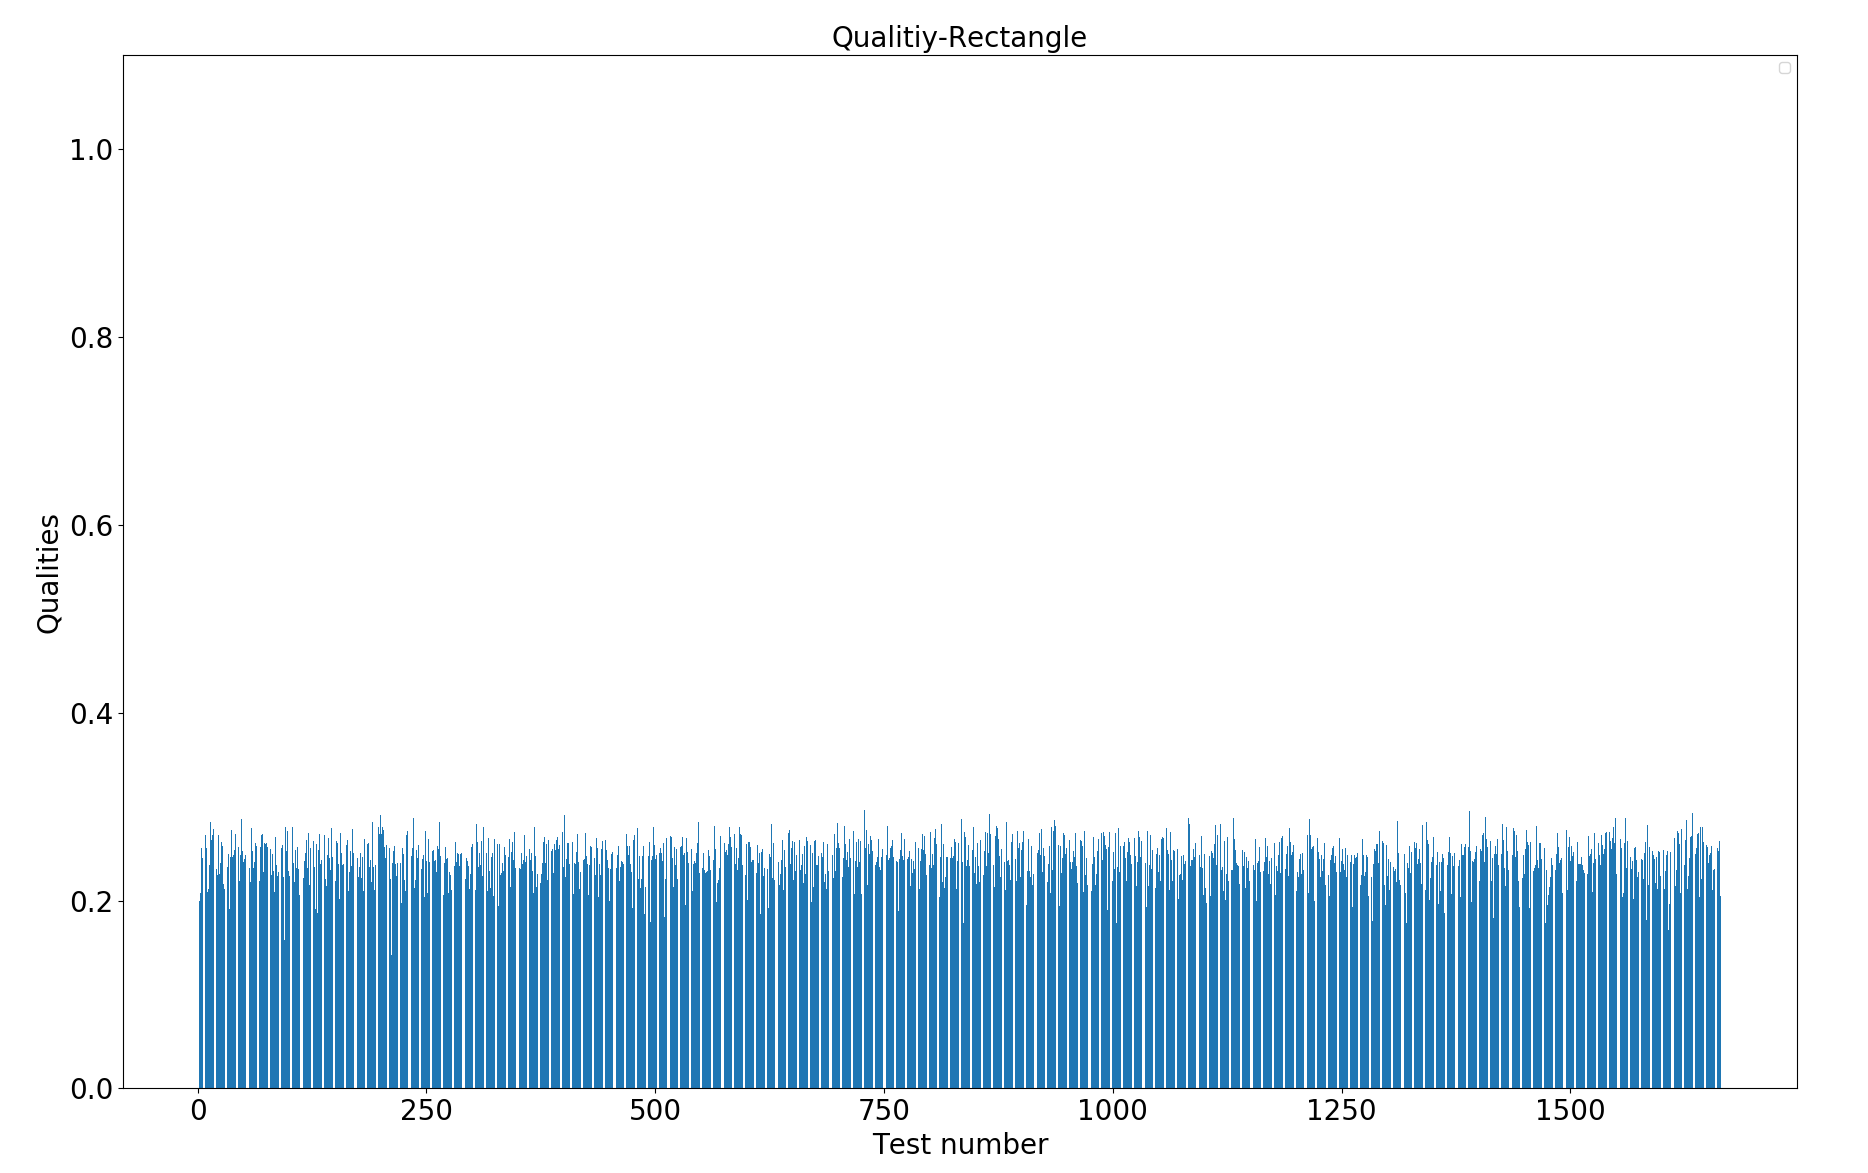
\includegraphics[width=\textwidth]{testQualities_Rectangle.png}\\
$\text{Qualité}_{rectangle} = \frac{\text{aire rectangle}}{\text{aire polygone}} - 100\%$\\
L'abscisse est représentée le numéro de test et l'ordonnée est la qualité de rectangle minimum convexe.
On peut voir que l'aire du rectangle minimum convexe est toujours plus grand que l'aire de polygone convexe.

\clearpage


\section{Algorithme Ritter}
\lhead{Calculer le cercle minimum convexe}
\subsection{Introduction}
Donner un ensemble $\mathcal{P}$ de n points dans $\mathbb{R}$, le cercle minimum convexe est le cercle qui entourne tous les points de $\mathcal{P}$ à la fois son aire est plus petit possible.\\
Pour calculer le cercle minimum convexe, il existe une majoration de $\mathcal{O}(n^4)$ en utilisant la recherche exhaustive. On énumère trois points pour déterminer un cercle, et vérifier s'il peut entourner tous les autres points.
Dans ce projet, j'utilise l'algorithme Ritter et cela me permet de résoudre ce problème en $\mathcal{O}(n)$.
\subsection{Présentation de l'algorithme Ritter}
Algorithme Ritter est proposé en 1990 par Jack Ritter afin de calculer efficacement la sphère minimum convexe. Cet algorithme peut évidemment calculer le cercle.

\begin{algorithm}
	$\mathcal{P} \gets \text{Ensemble de points}$\;
	$d \gets \text{point aléatoire}$\;
	$p \gets \text{le point plus éloigné de}$ $d$\;
	$q \gets \text{le point plus éloigné de}$ $p$\;
	$c \gets \frac{p + q}{2}$
	$Cer\gets Cercle(c,|cp|)$\;
	$\mathcal{P} \gets \mathcal{P}\setminus\{p, q\}$\;
	\While{$P \neq \varnothing$}{
		\For{ each Point $s$, $s\in\mathcal{P}$}{
			\If{$s \in Cer$ }{
				$\mathcal{P} \gets \mathcal{P}\setminus\{s\}$\;
			}
			\Else{
				$|st| \gets |cp| + |cs|$\;
				$|sc^{\prime}| \gets \frac{|st|}{2}$\;
				$c^{\prime} = c + \overrightarrow{cs}\cdot\frac{|sc| - |sc^{\prime}|}{|sc| + |cp|}$\;
				$Cer \gets new$ $Cercle(c^{\prime}, |sc^{\prime}|)$\;
			}
		}
	}
	\KwRet{$Cer$}\;
	\caption{Pseudocode de l'algorithme Ritter}
\end{algorithm}
\begin{enumerate}
	\item Choisir un point $d$ aléatoirement, $d\in\mathcal{P}$, chercher un point $p$ tel que la distance $|pd|$ est maximum.
	\item Chercher le point $q$, $q\in\mathcal{P}$ tel que la distance $|pq|$ est maximum. Construire un cercle $Cer$ par le point milieu $c$ entre $p$ et $q$ et le rayon $|cp|$.
	\item Enumérer tous les points $s$, $s\in\mathcal{P}$. Si $s$ est couvert par $Cer$, enlève $s$ directement.
	\item Sinon, on chercher un point $t$ sur $Cer$ tel que $t$ est le plus éloigné de $s$, $|st|$ passe $|sc|$. En plus calculer le point $c^{\prime}$ qui est le point milieu entre $s$ et $c$. Construire un nouveau cercle dont le rayon est $|c^{\prime}s|$ et le centre est $c^{\prime}$.\\
	Tips:\\
	$c^{\prime} = c + \overrightarrow{cs}\cdot\frac{|cc^{\prime}|}{|st|} = c + \overrightarrow{cs}\cdot\frac{|sc| - |sc^{\prime}|}{|sc| + |cp|} = c + \overrightarrow{cs}\cdot\frac{|sc| - |st|\times\frac{1}{2}}{|sc| + |cp|}$
	\item Remplacer $Cer$ par ce nouveau cercle centré en $c^{\prime}$.
	\item Tant que $\mathcal{P}\neq\varnothing$, retourne l'étape 3.
\end{enumerate}

\subsection{Performance de l'algorithme}
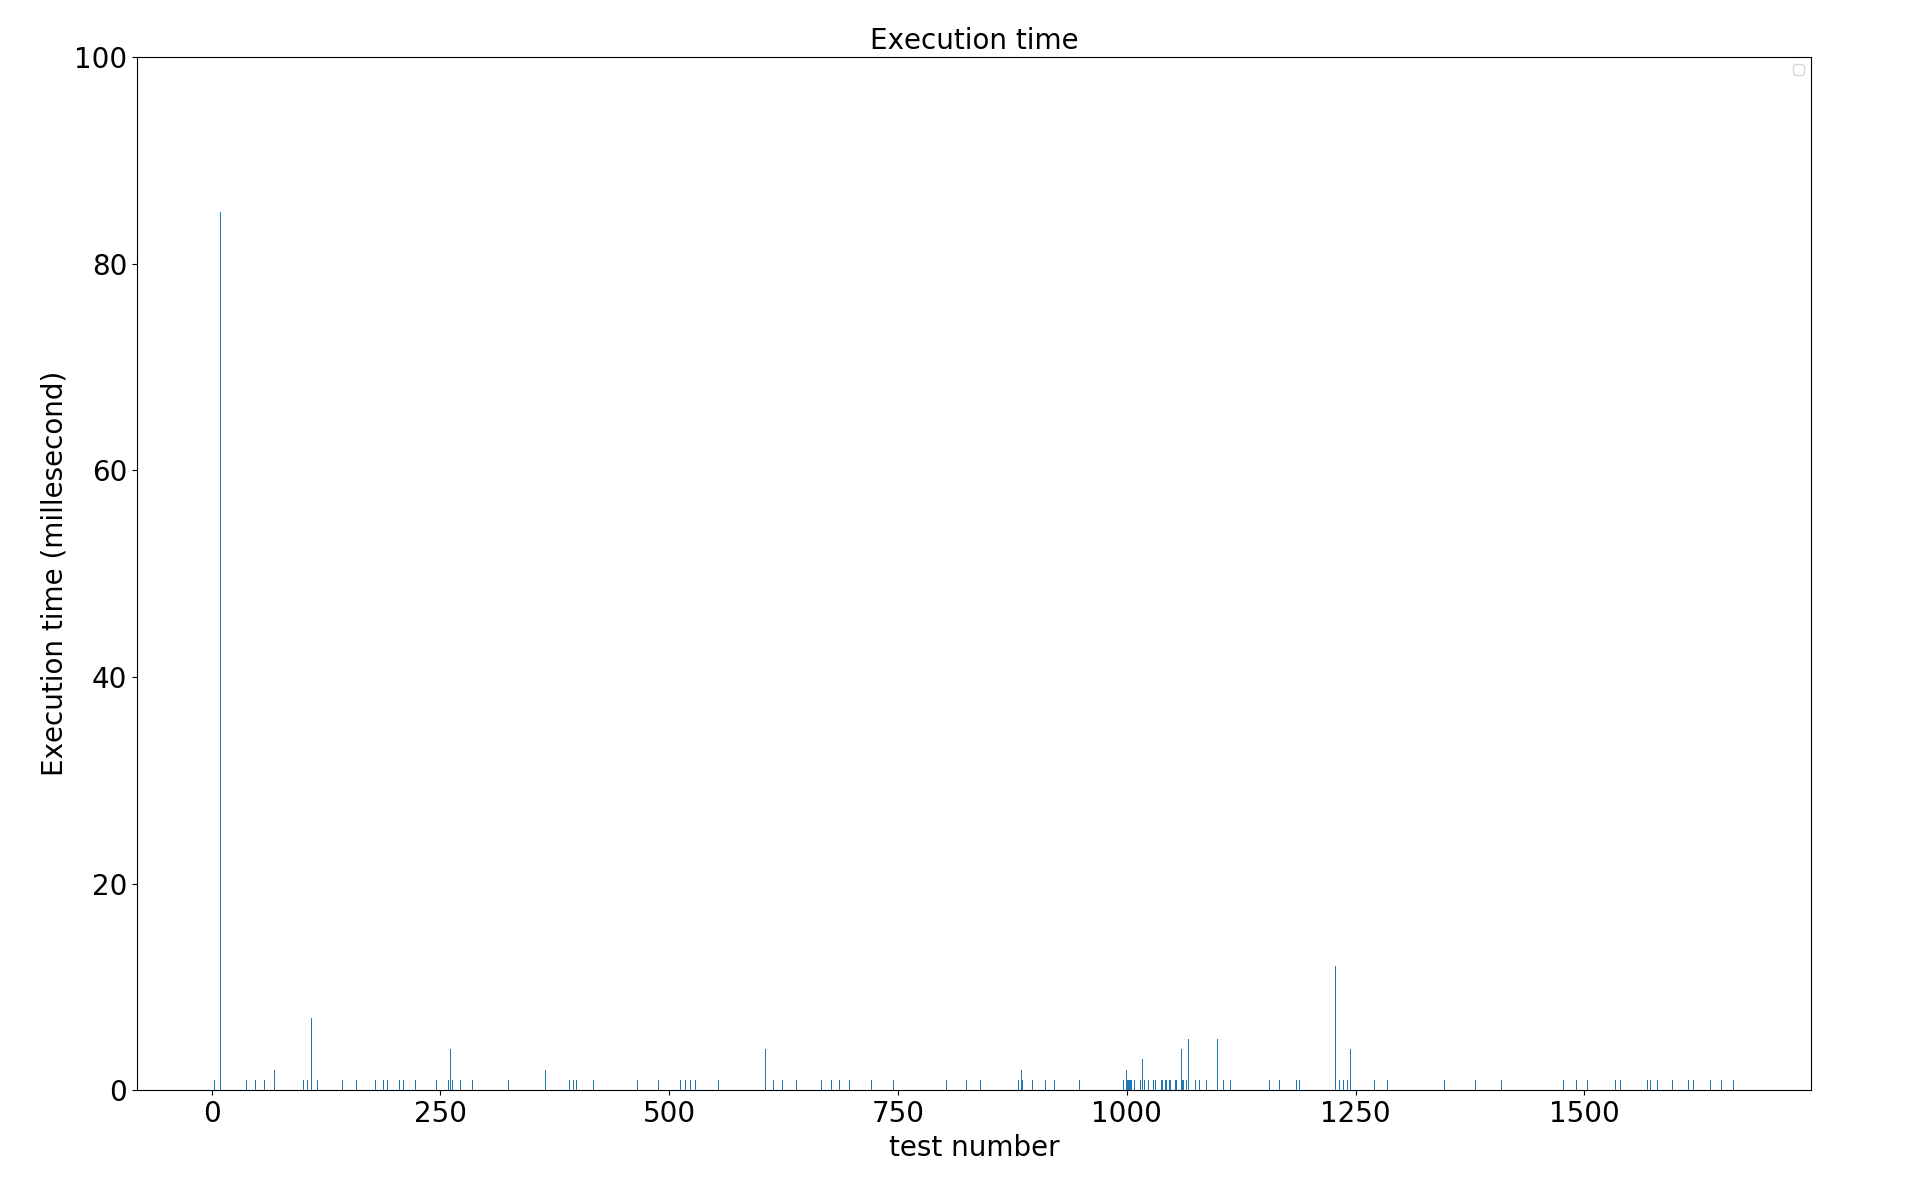
\includegraphics[width=\textwidth]{TestTime_Circle.png}\\
La complexité de l'algorithme Ritter est linéaire. Il y a $n$ points dans $\mathcal{P}$, au plus il fait seulement $n$ fois boucle pour enlever tous les points. Donc c'est linéaire. Néanmoins, cet algorithme utilise la fonction probabiliste afin d'optimiser sa performance, donc il nous permet seulement d'obtenir un résultat d’approximation au lieu d'une réponse parfaite.
Dans ces 1664 cas des tests, le test-10 coûte toujours le plus de temps 83 ms, mais les autres prennent seulement quelques millisecondes.

\subsection{Résultat du test}
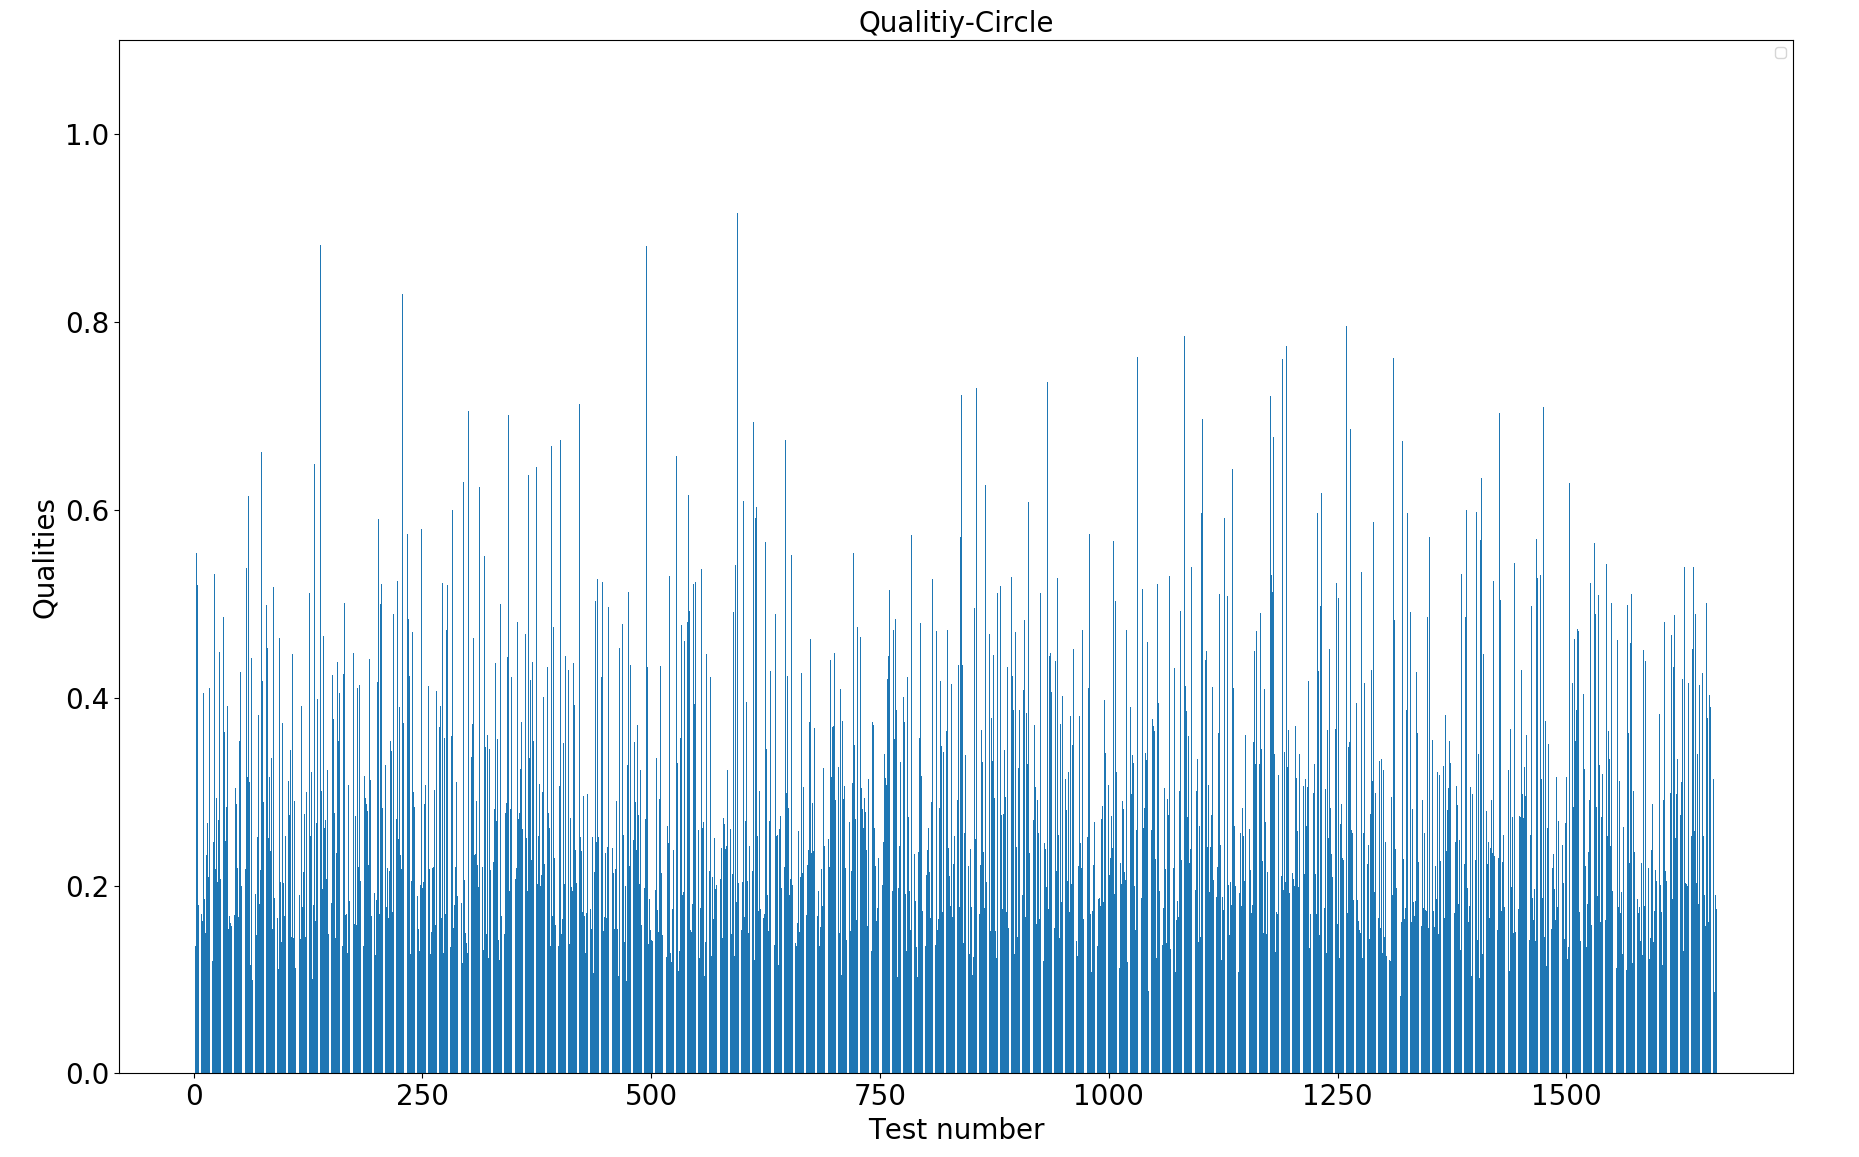
\includegraphics[width=\textwidth]{testQuality_Circle.png}\\
Le résultat obtenu par l'algorithme Ritter est approximatif, donc l'aire de cercle change toujours souvent, la qualité de cercle convexe n'est pas définitive.

\end{document}
